\section{Monte Carlo dataset}
The simulation used in this analysis is a PYTHIA6 production anchored to \pp\ data at $\s=7$~TeV.
The MC production is LHC15a2a (AOD produced together with ESD); the anchor data periods are LHC10b, LHC10c, LHC10d and LHC10e.
This MC production is anchored to the reconstruction pass 4.
This is a ``charm-enhanced'' production: 50\% of the events are required to have a \ccbar\ pair and the other half a \bbbar\ pair.
In addition all D mesons are forced to decay hadronically. The tune used in the production is Perugia2011 with the addition of the 
{\fontfamily{\ttdefault}kPyBeautyppMNRwmi} process.
The total number of analyzed events is 28.5 M. Results shown below come from the LEGO train Jets\_EMC\_pp\_MC, run n. 508.
\section{Overview of the analysis}
The \Dzero\ meson candidates are selected using the ``standard 2010 pp'' cuts, which are accessed through the static method AliRDHFCuts::SetStandardCutsPP2010(). Background is completely rejected by selecting only candidates that
have a MC label corresponding to a true generator-level \Dzero. In order to prepare the input for the jet finder, the daughters of the \Dzero\ mesons are 
removed from the charged particle collection (generator level) and from the track collection (detector level). The \Dzero\ particles and the \Dzero\ candidates are
added respectively to the charged particle collection and to the track collection. These collections are then used as inputs for the jet finder.
The jet finder algorithm is \antikt\ with a resolution parameter $R=0.6$ in its FastJet (v. 3.0.6) implementation.
Only jets containing a \Dzero\ meson are selected. For each particle-level and detector-level jet the following variable is calculated:
\begin{equation}
\zpar=\frac{\vec{p}_{\mathrm{ch.jet}}\cdot\vec{p}_{\mathrm{D}}}{\vec{p}_{\mathrm{ch.jet}}\cdot\vec{p}_{\mathrm{ch.jet}}}
\end{equation}
Detector-level jets are matched geometrically with particle-level jets. The distance between a particle-level jets and a detector-level jet is defined 
as the Euclidean measure in the $\left(\eta,\phi\right)$ plane. A detector-level jet is matched to its closest particle-level jet; however in order for this matching to be accepted
there mustn't be any other detector-level jet closer to the matched particle-level jet. These matching requirements have been used 
already in other jet measurements.

A 4-dimensional response matrix (\zpargen, \ptchjetgen, \zpardet, \ptchjetdet) is built by filling an entry for each successfully 
matched particle-level and detector-level jet pair. The particle-level unmatched jets that pass the kinematic and acceptance cuts
determine the amount of reconstruction inefficiency. The total reconstruction efficiency is mainly driven by
the D meson reconstruction efficiency, and to a less extent, by the jet reconstruction efficiency.

The main analysis tasks (C++ classes) used in the analysis are in the PWGJE library:
\begin{itemize}
\item AliAnalysisTaskSEDmesonsFilterCJ
\item AliAnalysisTaskDmesonJetCorrelations
\item AliJetResponseMaker
\end{itemize}
%%%%%%%%%%%%
%%%%%%%%%%%%
\section{Simulation figures}
%%%%%%%%%%%%
In the following paragraphs the 4 figures prepared for the Quark Matter 2015 conference are presented.
%%%%
\subsection{Jet reconstruction efficiency as a function of \zpargen\ in \ptchjetgen\ bins}
%%%%
Figure~\ref{fig:D0_Full_R060_Efficiency_Z_Vs_JetPt} shows the jet reconstruction efficiency as a function of \zpargen\ in 3 different \ptchjetgen\ bins,
compared with the \ptchjetgen\ integrated efficiency. The efficiency is taken as the ratio of the \zpar\ spectra of the particle-level jets for which a matched
detector-level jet was found over
all the particle-level jets (regardless of whether they are matched to a detector-level jet).
The same kinematical and acceptance cuts are applied to both numerator and denominator. The efficiency and its uncertainty is calculated
taking into account the fact that the numerator is a subset sample of the denominator. Bayesian inference has been used to calculate both
the efficiency and the errors using the root method TGraphAsymmErrors::Divide(...) with the option ``b(1,1) mode''.
\begin{figure}[tbh]
\begin{center}
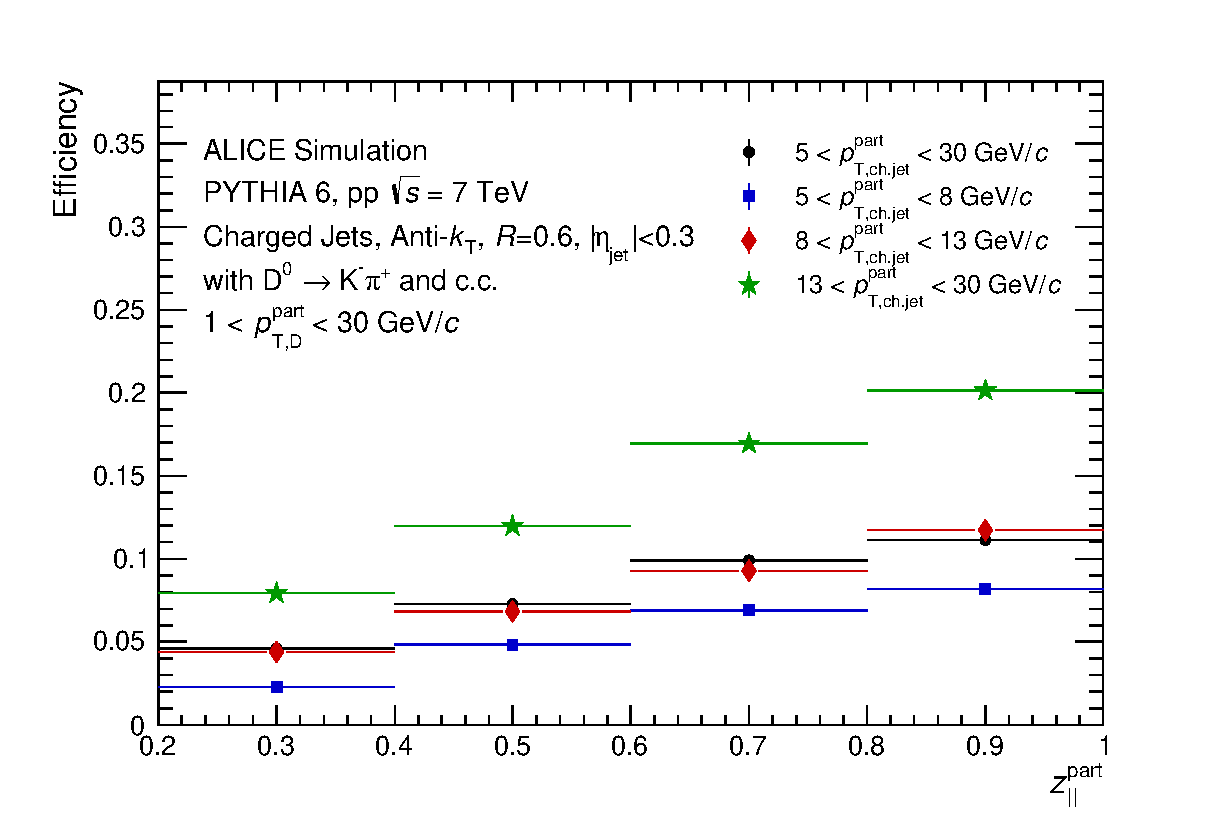
\includegraphics[width=0.8\textwidth]{img/D0_Full_R060_Efficiency_Z_Vs_JetPt}
 \caption{Jet reconstruction efficiency as a function of \zpargen\ in \ptchjetgen\ bins.} 
 \label{fig:D0_Full_R060_Efficiency_Z_Vs_JetPt}
\end{center}
\end{figure}
%%%%
\subsection{Jet reconstruction efficiency as a function of \zpargen\ in \ptdgen\ bins}
%%%%
Figure~\ref{fig:D0_Full_R060_Efficiency_Z_Vs_JetPt} shows the jet reconstruction efficiency as a function of \zpargen\ in 6 different \ptdgen\ bins,
compared with the \ptdgen\ integrated efficiency. The same procedure as the one described in the previous paragraph has been used to generate
this efficiency.
\begin{figure}[tbh]
\begin{center}
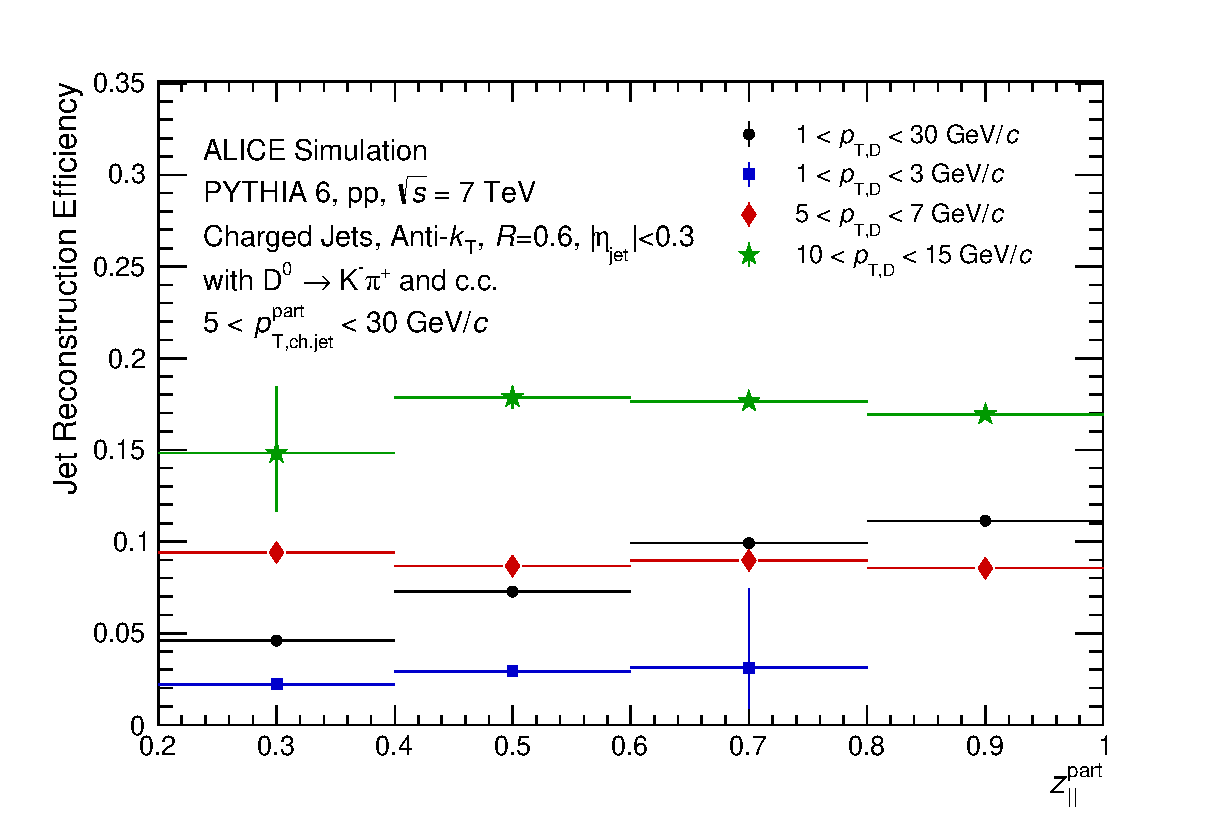
\includegraphics[width=0.8\textwidth]{img/D0_Full_R060_Efficiency_Z_Vs_DPt}
 \caption{Jet reconstruction efficiency as a function of \zpargen\ in \ptdgen\ bins.} 
 \label{fig:D0_Full_R060_Efficiency_Z_Vs_DPt}
\end{center}
\end{figure}
%%%%
\subsection{Response matrix for \ptchjet\ (\zpar\ integrated)}
%%%%
Figure~\ref{fig:D0_Full_R060_ResponseMatrix_JetPt_Z_20_100_DPt_01_30_Norm} shows the response matrix (\ptchjetgen, \ptchjetdet), obtained by
projecting the 4-dimensional response matrix (\zpargen, \ptchjetgen, \zpardet, \ptchjetdet), i.e. integrating in both \zpargen and \zpardet.
\begin{figure}[tbh]
\begin{center}
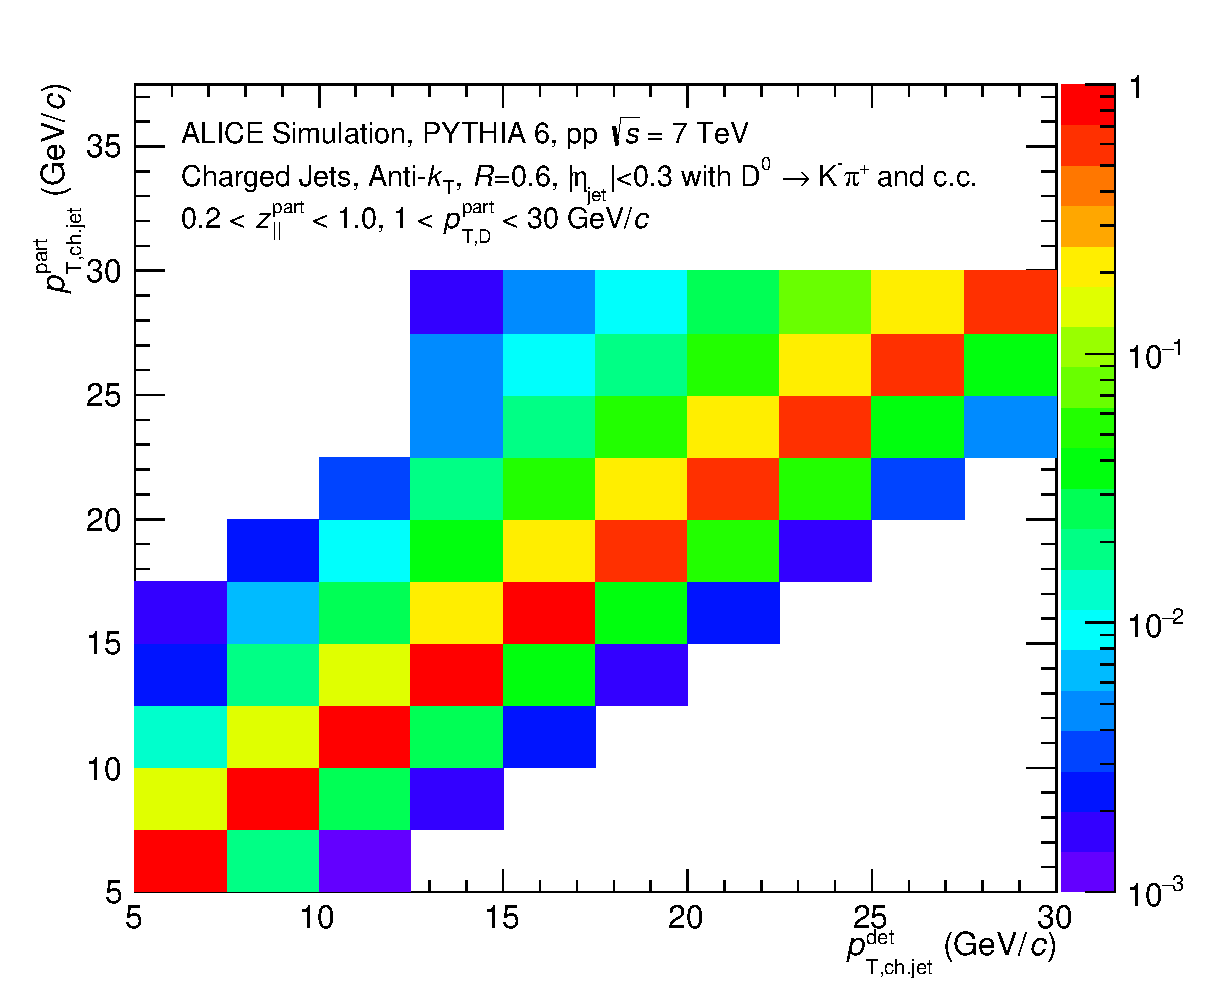
\includegraphics[width=0.8\textwidth]{img/D0_Full_R060_ResponseMatrix_JetPt_Z_20_100_DPt_01_30_Norm}
 \caption{Response matrix for \ptchjet\ (\zpar\ integrated).} 
 \label{fig:D0_Full_R060_ResponseMatrix_JetPt_Z_20_100_DPt_01_30_Norm}
\end{center}
\end{figure}
%%%%
\subsection{Response matrix for \zpar\ (with $5<\ptchjetgen<8$~\GeVc)}
%%%%
Figure~\ref{fig:D0_Full_R060_ResponseMatrix_Z_JetPt_5_8_DPt_01_30_Norm} shows the response matrix (\zpargen and \zpardet), obtained by
projecting the 4-dimensional response matrix (\zpargen, \ptchjetgen, \zpardet, \ptchjetdet), i.e. integrating in $5<\ptchjetgen<8$~\GeVc\ and in  \ptchjetdet over the
full range.
\begin{figure}[tbh]
\begin{center}
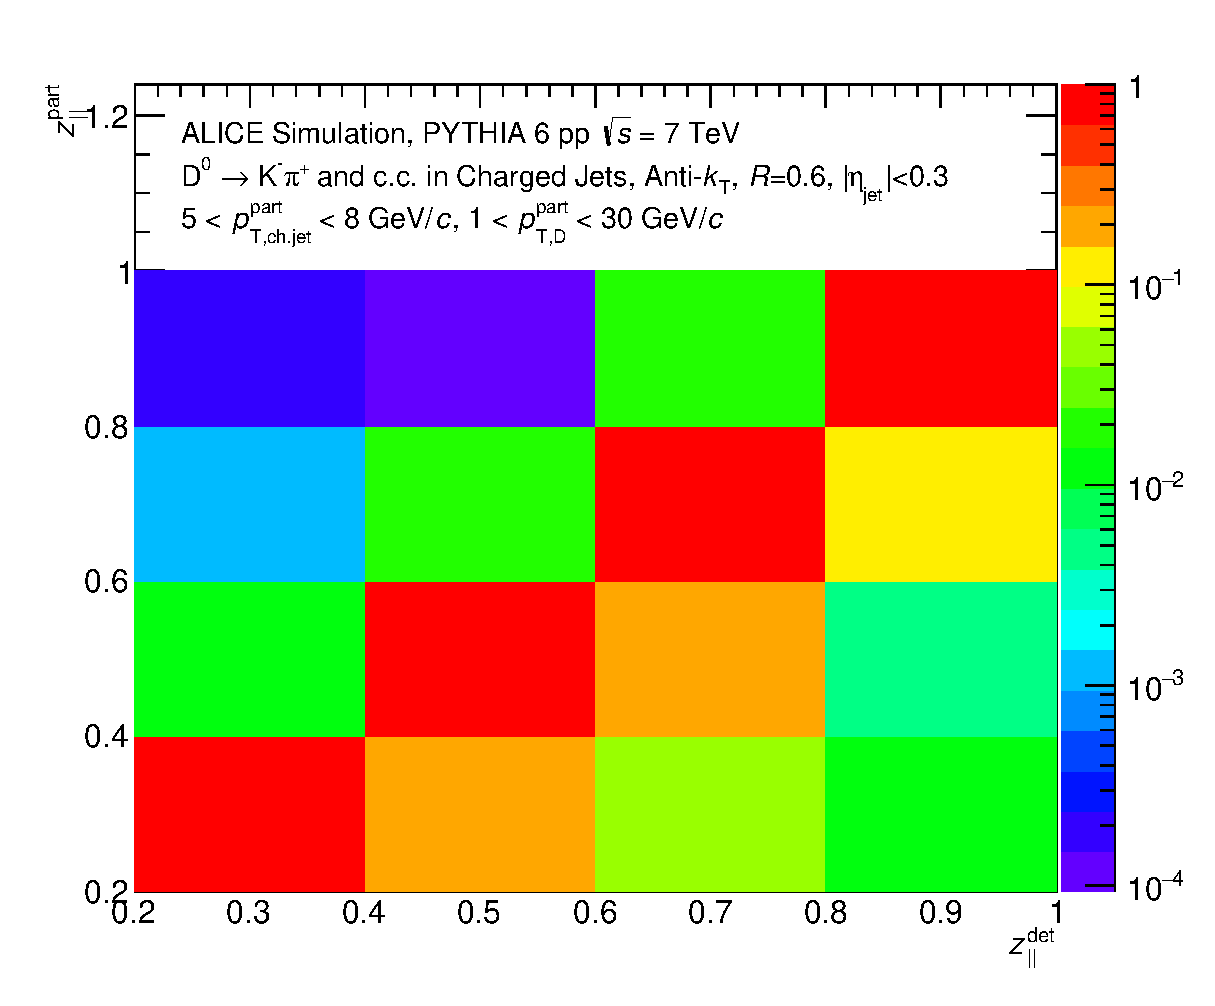
\includegraphics[width=0.8\textwidth]{img/D0_Full_R060_ResponseMatrix_Z_JetPt_5_8_DPt_01_30_Norm}
 \caption{Response matrix for \zpar\ (with $5<\ptchjetgen<8$~\GeVc).} 
 \label{fig:D0_Full_R060_ResponseMatrix_Z_JetPt_5_8_DPt_01_30_Norm}
\end{center}
\end{figure}
